\chapter{Обзор предметной области}\label{ch:ch1}

\section{Генетические и эпигенетические факторы}\label{sec:ch1/sec1}

\subsection{Виды и структура ДНК}\label{subsec:ch1/sec1/subsec1}

Дезоксирибонуклеиновая кислота (ДНК) обеспечивает реализацию и передачу из поколения в поколение генетической информации, касающейся развития, функционирования, роста и размножения живых организмов. Такие основные понятия современной генетики, как наследственность и изменчивость, связаны с молекулами ДНК. Наследственность определяют как способность живых организмов передавать свои признаки потомству, а изменчивость --- как способность приобретать отличия, обеспечивая тем самым биоразнообразие \autocite{rieger2012glossary}. 

ДНК представляет собой макромолекулу, состоящую из двух цепей нуклеотидов \autocite{brooker2004genetics,lesk2017introduction}. Эти цепи, закручиваясь друг вокруг друга, при помощи водородных связей образуют двойную спираль. Две цепи ДНК состоят из нуклеотидов, каждый из которых состоит из фосфатной группы, сахара (дезоксирибозы) и одного из четырёх азотистых оснований --- цитозин (C), гуанин (G), аденин (A) или тимин (T) \autocite{alberts2008molecular,berg2010biochemistry}. Каждое из оснований на одной цепи ДНК связано с определённым основанием на второй цепи по правилу комплементарности: цитозин связывается только с гуанином, аденин --- с тимином \autocite{tropp2012molecular}. Это означает, что вся информация, которую несёт одна цепь, дублируется на второй цепи. Такое специфическое обратимое взаимодействие имеет крайне важное значение для всех функций ДНК в живых организмах \autocite{alberts2017molecular}. 

Внутри ядер клеток эукариот располагается ядерная ДНК, структурированная в длинные структуры --- хромосомы. В ядрах клеток организма содержится человека 46 индивидуальных хромосом. Ядерная ДНК может существовать в нескольких копиях, число которых определяет термин <<плоидность>> \autocite{brown2002genomes,alberts2017molecular}. Соматические клетки человека диплоидны, то есть содержит две копии каждой хромосомы (всего 23 пары). Наследование ядерной ДНК является биродительским, то есть каждая из двух копий генома наследуется от одного из родителей --- матери или отца. 

Генетическая информация хранится в генах, а совокупность всех генов в организме называется его генотипом. Ген --- это единица наследственности и область ДНК, которая влияет на определённые характеристики организма. Ядерная ДНК человека содержит около 25000 генов, однако, более 98\% генома не кодируют генетическую информацию \autocite{Wolfsberg2001}. Распространённой формой некодирующей ДНК у людей являются псевдогены, которые представляют собой копии генов, утративших функциональность в результате мутации \autocite{Harrison2002}.

В клетках эукариот ДНК располагается не только в ядрах, но и в митохондриях, клеточных органеллах, окисляющих органические соединения для преобразования высвобождающейся энергии в аденозинтрифосфат (АТФ). Митохондриальная ДНК была первой секвенированной частью генома, она состоит из 16569 пар оснований и кодирует 13 белков \autocite{Anderson1981}, некодирующие участки отсутствуют. Она в большей степени подвержена мутациям в сравнении с ядерной ДНК. Митохондриальная ДНК представляет собой двухцепочечную кольцевую молекулу ДНК, организованную в хромосому. Большинство белков, необходимых митохондриям, кодирует митохондриальная ДНК, остальная часть кодируется ядерной ДНК. В свою очередь, ядерная ДНК кодирует все белки, требуемые клетке. Одна митохондрия содержит несколько десятков копий митохондриальной ДНК. Поскольку в одной клетке может находиться более 100 митохондрий, общее число копий митохондриальной ДНК превышает 1000 на одну клетку \autocite{lodish2012molecular}. 

Митохондриальная ДНК наследуется по материнской линии, поскольку цитоплазма в зиготу поступает только от яйцеклетки. Следовательно, заболевания, связанные с митохондриальной ДНК, передаются по наследству от матери \autocite{cooper2004cell}. Самый последний общий предок по материнской линии всех современных людей называют Митохондриальной Евой. Группа схожих гаплотипов (унаследованных от одного родителя аллелей), имеющих общего предка с определённой мутацией, называется гаплогруппой. Гаплогруппы относятся к одной линии наследования \autocite{cox2016biogeography}. То есть членство любого человека в гаплогруппе зависит от относительно небольшой части генетического материала, которым обладает этот человек. Каждая гаплогруппа происходит от одной предыдущей гаплогруппы и остаётся ее частью. Таким образом, любая родственная группа гаплогрупп моделируется как вложенная иерархия, в которой каждый набор (гаплогруппа) является подмножеством одного более широкого набора \autocite{Arora2015}. На вершине данной иерархии и располагается Митохондриальная Ева. Гаплогруппы обычно обозначаются заглавной буквой алфавита, а уточнения состоят из дополнительных комбинаций цифр и букв, например, $A \rightarrow A1 \rightarrow A1a$.

Изучением генов, генетической изменчивости и наследственности живых организмов занимается генетика \autocite{griffiths2000introduction}. Современная генетика вышла за рамки наследования и занимается также изучением функций и поведения генов в масштабах клетки, организма и популяции. Генетика дала начало ряду подразделов, включая молекулярную генетику, эпигенетику и популяционную генетику.

\subsection{Метилирование ДНК}\label{subsec:ch1/sec1/subsec2}

Фенотип организма характеризует физическую форму, структуру организма, его процессы развития, биохимические и физиологические свойства, поведение и многое другое. Фенотип определяется двумя основными факторами: генотип организма (совокупность всего генетического кода) и влиянием факторов окружающей среды. Оба фактора могут взаимодействовать, дополнительно влияя на фенотип \autocite{Dawkins2010}. В биологии эпигенетика изучает наследственные изменения фенотипа, не связанные с изменением последовательности ДНК \autocite{Dupont2009}. Эпигенетика чаще всего исследует изменения, которые влияют на активность и экспрессию генов, но этот термин также может использоваться для описания любых наследственных фенотипических изменений. Такое воздействие на клеточные и физиологические фенотипические признаки может быть результатом как внешних факторов, так и факторов окружающей среды или быть частью нормального развития. Эпигенетика также относится к функционально значимым изменениям в геноме, которые не связаны с изменением нуклеотидной последовательности. Наиболее известным примером механизма, вызывающего такие изменения, является метилирование ДНК, которое изменяет экспрессию генов без изменения последовательности ДНК \autocite{Bird2007}. Экспрессия генов может контролироваться действием специальных белков-репрессоров, прикрепляющихся к сайленсерам ДНК --- регионам, связывание с которыми приводит к снижению или подавлению синтеза РНК \autocite{Pang2020}.

Метилирование ДНК --- это биологический процесс, с помощью которого к молекуле ДНК добавляются метильные группы. Метилирование может изменить активность сегмента ДНК без изменения последовательности --- находясь в промоторе гена (стартовый регион гена для начала транскрипции), оно обычно подавляет транскрипцию гена. Метилировано может быть только одно из четырёх оснований ДНК --- цитозин, располагающийся в динуклеотиде CG (положение нуклеотидов в цепи ДНК, при котором в линейной последовательности за нуклеотидом C следует нуклеотид G) \autocite{BuckKoehntop2013, Kelsey2013}. Обычно их называют сайтами CpG.

У млекопитающих существуют регионы ДНК, богатые на CpG сайты --- эти области называются островами CpG \autocite{Bird1986}. Они определяются как регионы длиной более 200 bp (спаренных оснований), с содержанием динуклеотидов CG более $50~\%$ и отношением ожидаемого количества CpG сайтов к реальному больше $0.6$ \autocite{GardinerGarden1987}. Пример острова CpG приведён на рисунке~\cref{fig:CpG_Island}. В геноме человека имеется около 25000 островов CpG, $75~\%$  которых имеют длину менее 850 пар оснований \autocite{Lander2001}. Они являются основными регуляторными единицами, и около $50~\%$ островков CpG расположены в областях промоторов генов. В свою очередь, около $60-70~\%$ генов человека имеют остров CpG в своей промоторной области \autocite{Illingworth2010, Saxonov2006}.

\begin{figure}[ht]
	\centerfloat{
		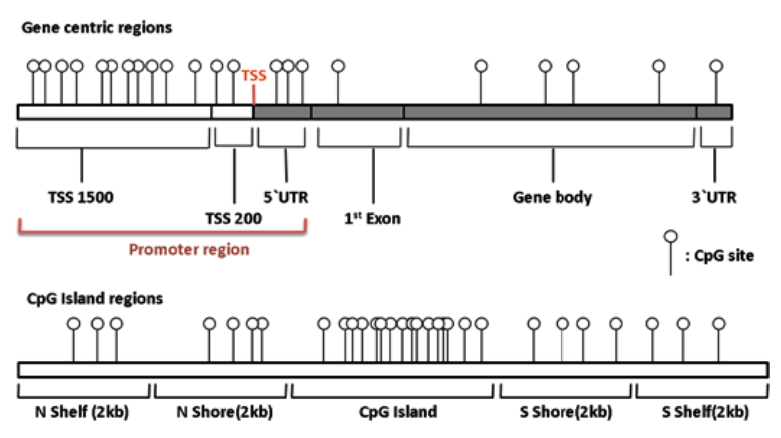
\includegraphics[scale=0.7]{island.png}
	}
	\caption[Пример острова CpG, региона с самой высокой плотностью размещения сайтов CpG в промоторной области гена.]{Пример (верх) генных регионов, (низ) острова CpG (CpG island). Промоторная область гена состоит из регионов TSS1500, TSS200, 5'UTR, далее следуют 1stExon, тело гена и 3'UTR. Остров CpG --- регион с самой высокой плотностью размещения сайтов CpG в промоторной области гена. По обе стороны от острова CpG располагаются побережья (CpG shore), регионы с меньшей плотностью размещения сайтов CpG, далее --- шельфы, регионы с малой плотностью размещения сайтов CpG \autocite{Wijnands2016}.}\label{fig:CpG_Island}
\end{figure}

Метилирование ДНК может быть обнаружено с помощью различных техник и анализов, таких как масс-спектрометрия, бисульфитное секвенирование генома, анализ кривых плавления с высоким разрешением, технология Illumina \autocite{Rana2018}. Масс-спектрометрия является чувствительным и надёжным методом детектирования метилирования ДНК, однако, этот метод не информативен при исследовании метилирования в контексте последовательности, что является значительным ограничением. Бисульфитное секвенирование генома (BS-Seq) представляет собой высокопроизводительный анализ метилирования в масштабах всего генома. Он основан на конверсии геномной ДНК бисульфитом натрия, которая превращает неметилированные цитозины динуклеотидов CpG в урацил (UpG), а метилированные цитозины при этом не изменяются \autocite{Hernandez2013}. Полученный геном секвенируется на платформах нового поколения, и производится сравнение с исходным геномом для выявления несоответствий. Анализ кривых плавления высокого разрешения основывается на том, что бисульфит-конвертированные высокометилированные последовательности ДНК имеют другую температуру плавления по сравнению с неметилированными \autocite{Malentacchi2009}. Данный метод используется для определения количественной оценки уровня метилирования. Одним из наиболее распространённых методов является технология компании Illumina. Illumina Methylation Assay измеряет метилирование ДНК на каждом локусе с использованием матричной гибридизации. Бисульфит-конвертированная ДНК гибридизируется на специальных чипах «BeadChips». Основными чипами являются 27K Illumina HumanMethylation array и Infinium HumanMethylation450 BeadChip, измеряющие уровень метилирования на 27000 и 450000 сайтах CpG, соответственно. В 2016 году был выпущен чип Infinium MethylationEPIC BeadChip, который измеряет уровень метилирования на 850000 сайтов CpG в геноме человека.

Метилирование ДНК может влиять на транскрипцию генов двумя способами. Во-первых, метилирование ДНК может физически препятствовать связыванию транскрипционных белков с геном \autocite{Choy2010}, во-вторых, сайты CpG могут связываться с белками, известными как метил-CpG-связывающие домены (MBD --- Methyl-CpG-binding domain). Эти белки участвуют в формировании гетерохроматина --- участка хроматина (основы хромосомы) с низкой транскрибируемостью (возможность переноса генетической информации с ДНК на РНК). 

Почти все паттерны метилирования, наследованные от родителей, стираются во время гаметогенеза и в раннем эмбриогенезе. После имплантации эмбриона паттерны метилирования зависят от стадии развития и ткани, а изменения в метилировании каждого отдельного типа клеток стабильно сохраняются на достаточно долгий период \autocite{Cedar2012}. Во время эмбрионального развития немногие гены изменяют свой статус метилирования, за исключением тех генов, которые экспрессируются исключительно у зародышей \autocite{Borgel2010}.

При многих заболеваниях, таких как, например, рак, острова CpG промотора гена становятся аномально гипометилированы, что приводит к подавлению транскрипции \autocite{Wang2018Cancer}. Важным компонентом развития онкологических заболеваний являются изменения в метилировании ДНК. Как правило, при прогрессировании рака активность многих генов либо подавляется, либо активируется. Несмотря на то, что подавление некоторых генов при раке происходит в результате мутаций, большая часть подавленных канцерогенных генов является результатом изменённого метилирования ДНК. 

Такие эпигенетические модификации как метилирование ДНК, также тесно связаны с сердечно-сосудистыми заболеваниями, включая атеросклероз. Гипометилирование ДНК влияет на гены, которые вызывают дисфункцию эндотелиальных клеток (выстилающих внутреннюю поверхность кровеносных и лимфатических сосудов) и увеличивают количество <<медиаторов воспаления>>, что значительным образом влияет на формирование атеросклеротических поражений \autocite{Castro2003}. 

В процессе старения происходит накопление эпигенетических изменений, в частности, глобальное изменение метилирования ДНК. Уровень метилирования различных тканей и органов человека можно использовать для оценки его биологического возраста с помощью, например, эпигенетических часов \autocite{Horvath2013}. 

\subsection{Эпигенетические биомаркеры старения человека}\label{subsec:ch1/sec1/subsec3}

Старение --- сложное ухудшение физиологических процессов с течением времени, происходящее в большинстве живых организмов \autocite{rose1994evolutionary}. Учёные предложили девять признаков старения, которые можно разделить на три категории: первичные, антагонистические и интегративные \autocite{LopezOtin2013}. К первичным признакам относятся нестабильность генома, укорочение теломер, эпигенетические изменения, потеря протеостаза; к антагонистическим --- нарушение распознавания питательных веществ, митохондриальная дисфункция, клеточное старение; к интегративным --- истощение пула стволовых клеток, изменение межклеточного взаимодействия. 

Биомаркеры старения --- это биомаркеры, которые могут прогнозировать функциональную способность отдельных органов и всего организма в целом в более позднем возрасте лучше, чем хронологический возраст \autocite{Baker1988}. Другими словами, биомаркеры старения показывают истинный «биологический возраст», который может отличаться от хронологического возраста. Подтверждённые биомаркеры старения позволят тестировать подходы к увеличению продолжительности жизни. Однако, несмотря на то, что максимальная продолжительность жизни была бы хорошим средством проверки биомаркеров старения, это не подходит для долгоживущих видов, потому что исследования потребовали бы слишком много времени. В идеале биомаркеры старения должны анализировать именно биологический процесс старения, а не предрасположенность к определённым заболеваниям, должны воспроизводиться в течение короткого интервала времени по сравнению с продолжительностью жизни организма.

Распространённое использование данных метилирования ДНК в качестве биомаркеров старения --- построение эпигенетических часов, позволяющий оценить биологический возраст любой ткани организма на протяжении всей жизни \autocite{Horvath2018}. ДНК в лейкоцитах, как правило, гипометилирована с возрастом, в то время как конкретные сайты CpG в промоторах генов имеют тенденцию быть гиперметилированными \autocite{Heyn2012, Gentilini2012}. Существует метод определения биологического возраста, основанный на паттернах метилирования конкретных сайтов CpG, со средней точностью $\pm~3.6$ года с корреляцией $0.96$. Из 353 сайтов CpG 193 оказались гиперметилированными, а 160 --- гипометилированными с возрастом \autocite{Horvath2013}. Связанное с возрастом гиперметилирование преимущественно затрагивает гены, участвующие в контроле метаболизма \autocite{Gentilini2012, Christensen2009}. Напротив, гипометилирование связано с повторяющимися элементами последовательности ДНК, например, Alu-повтор \autocite{Gentilini2012}.

Ряд эпидемиологических исследований показал, что монозиготные близнецы демонстрируют повышенный уровень фенотипического несоответствия, особенно в отношении возрастных заболеваний \autocite{Frederiksen2002, Reynolds2005, Zwijnenburg2010, CastilloFernandez2014}. Это может быть связано с постепенным увеличением скорости изменения метилирования при делении клеток \autocite{Issa2014}. Сравнение старых и молодых монозиготных пар близнецов показывает наличие глобальных различий в паттернах метилирования \autocite{Levesque2014, Tan2016, Wang2018Twins}. Также было показано, что метилом столетнего человека в среднем демонстрирует снижение как уровней метилирования ДНК, так и парных корреляций для соседних CpG сайтов в сравнении с новорождёнными \autocite{Heyn2012}. Мононуклеарные клетки периферической крови итальянских долгожителей (105-109 лет) имели эпигенетический профиль на $8.6$ лет моложе ожидаемого, а их дети (50–89 лет) имели эпигенетический возраст на $5.1$ года меньше, чем контрольная группа того же возраста \autocite{Horvath2015}.

Изменения в метилировании ДНК могут быть обусловлены как генетическими факторами, так и факторами окружающей среды, помимо самого старения. Внешние факторы окружающей среды, такие как, например, курение, пребывание на солнце и ожирение, связаны со специфическими изменениями в паттернах метилирования ДНК \autocite{Gronniger2010, Breitling2011, Almen2014, Vandiver2015}. Важно отметить, что конкретные генетические мутации, встречающиеся с разной частотой или включающие популяционные взаимодействия генов и окружающей среды, могут приводить к этническим различиям в паттернах метилирования ДНК \autocite{Galanter2017, Fagny2015, Heyn2013} и стимулируют различные модели эпигенетического старения. 

Первыми обнаруженными биомаркерами, имеющими высокий уровень корреляции с возрастом, были сайты CpG, располагающиеся в генах ELOVL2, FHL2 и PENK \autocite{Garagnani2012}. В данном исследовании проводился анализ профилей метилирования цельной крови людей в возрасте от 9 до 83 лет (матерей и их детей) с использованием чипа Illumina Infinium HumanMethylation450 BeadChip. Корреляционный анализ Спирмена показал высокие значения коэффициента корреляции между уровнями метилирования и возрастом субъектов. Острова CpG генов ELOVL2, FHL2 и PENK, расположенные в промоторных областях, демонстрируют гиперметилирование с увеличением хронологического возраста, как изображено на рисунке~\cref{fig:ELOVL2}. Впоследствии было показано, что корреляция с возрастом уровня метилирования проб в гене ELOVL2 не является специфичной для цельной крови, а наблюдается также в тканях мозга, кожи, подкожно-жировой клетчатки, печени, щитовидной железы \autocite{Slieker2018}, и, более того, не является специфичной для человека, а наблюдается также, например, у мышей \autocite{Spiers2016}. Тем не менее, большинство коррелирующих с возрастом сайтов CpG являются тканеспецифичными.

\begin{figure}[ht]
	\centerfloat{
		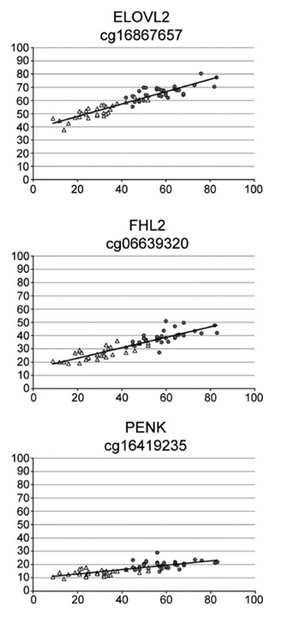
\includegraphics[scale=0.95]{elovl.png}
	}
	\caption[Зависимость уровней метилирования от возраста для сайтов CpG, имеющих наиболее высокое значение коэффициента корреляции.]{Зависимость уровней метилирования от возраста для сайтов CpG, имеющих наиболее высокое значение коэффициента корреляции. Точками отмечены уровни метилирования матерей, треугольниками --- детей \autocite{Garagnani2012}.}\label{fig:ELOVL2}
\end{figure}

В дополнение к изменению уровня метилирования ДНК с возрастом, существуют также стохастические эпигенетические мутации (эпимутации), которые случайным образом возникают в геноме и не распространяются среди субъектов. Теория соматических мутаций утверждает, что накопление стохастических мутаций в соматических клетках приводит к снижению клеточных функций \autocite{Kennedy2012} и играют важную роль при старении и развитии некоторых возрастных заболеваний. В работе \autocite{Gentilini2015} в популяции нормальных субъектов для каждого сайта CpG цельной крови был оценён нормальный диапазон уровня метилирования. Если значение уровня метилирования у конкретного субъекта выходило за границы нормального диапазона и было чрезвычайно далеко от такового у других субъектов, то в данном CpG сайте присутствует эпимутация. Было показано, что количество стохастических эпигенетических мутаций невелико в детстве и экспоненциально увеличивается с возрастом. 

Однако, в качестве независимой переменной в анализе уровней метилирования ДНК можно рассматривать не только возраст, но и другие характеристики, например, пол, индекс массы тела, наличие вредных привычек и многие другие.

\subsection{Гендерные различия уровней метилирования ДНК}\label{subsec:ch1/sec1/subsec4}

С биологической точки зрения пол у конкретного вида определяется размером гамет: организмы с большими гаметами являются самками, с маленькими --- самцами \autocite{smith1978evolution}. Хорошо известно, что мужчины и женщины отличаются на метаболическом уровне. Например, было обнаружено, что женщины более чувствительны к инсулину, они имеют более низкие уровни липопротеинов низкой плотности в плазме и более высокие уровни липопротеинов высокой плотности по сравнению с мужчинами \autocite{Freedman2004, Magkos2007}. Кроме того, пол может влиять на риск, возраст начала и симптомы заболевания \autocite{Kim2010}. Поэтому важно определить молекулярные механизмы, которые способствуют возникновению этих различий между мужчинами и женщинами. Половые различия связаны не только с половыми хромосомами и гормонами, но и с различиями в экспрессии генов и эпигенетических паттернах \autocite{Mittelstrass2011, Hall2014}. Существуют исследования, рассматривающие гендерные эпигенетические особенности в различных тканях и органах \autocite{Liu2010, Boks2009}. 

Половые различия существуют как в структуре и функциях мозга, так и в степени подверженности неврологическим расстройствам. Например, когнитивные функции, такие как память и внимание, у мужчин и женщин различаются \autocite{Gur1999}. Однако, молекулярная основа различий в восприятии, познании, памяти и нервных функциях мужчин и женщин изучена недостаточно. Есть предположение, что половые различия в функции мозга могут быть связаны с генетическими мутациями \autocite{Qureshi2010} и факторами окружающей среды, такими как пренатальный стресс \autocite{Bowman2004} или гормональный фон \autocite{Lenz2010}.

В работе \autocite{Xu2013} различия в уровне метилирования ДНК префронтальной коры головного мозга были распределены, в основном, по X хромосоме ($92.4~\%$ сайтов CpG, имеющих различный уровень метилирования у мужчин и женщин). Более $65~\%$ сайтов CpG были гиперметилированы у женщин в сравнении с мужчинами. Похожие результаты были получены для пуповинной крови новорождённых с поправкой на клеточный состав \autocite{Yousefi2015}. Гендерные различия в уровне метилирования аутосомной ДНК (не половые хромосомы) стабильны во времени и не зависят от популяционной принадлежности. В образцах цельной крови в генах CISH и RAB23 были найдены различно метилированные сайты CpG у мужчин и женщин, которые приводили к гендерным различиям в экспрессии данных генов \autocite{Singmann2015}. Они демонстрировали более низкие уровни метилирования у женщин по сравнению с мужчинами. Во многих из этих исследований анализировалось только ограниченное количество генов и их участков, таких как промоторная область, и не проводился полногеномный анализ метилирования ДНК.

Анализ гендерных различий уровня метилирования ДНК в масштабах всего генома проводится с помощью Infinium HumanMethylation450 BeadChip. Первое полногеномное исследование сообщило, что существуют как хромосомные, так и специфические для конкретного сайта CpG половые различия в метилировании ДНК на хромосоме X островков поджелудочной железы человека. Однако, аутосомные хромосомы показали гендерные различия в метилировании ДНК только на уровне отдельных CpG-сайтов. Также была обнаружена более высокая секреция инсулина в островках поджелудочной железы у женщин по сравнению с мужчинами и различия в экспрессии генов \autocite{Hall2014}. Половые различия метилирования ДНК клеток печени также были найдены в хромосоме X и аутосомах, как по всей хромосоме, так и по отдельным сайтам CpG. У женщин наблюдалась более высокая экспрессия гена KDM6A и APOA1, подавление которых может способствовать снижению уровня липопротеинов высокой плотности \autocite{GarciaCalzon2018}.

Пол оказывает влияние также на различия в морфологии и метаболизме скелетных мышц \autocite{Haizlip2015, Lundsgaard2014}, на возрастное сокращение мышц и их ремоделирование \autocite{Gheller2016}. Стволовые клетки взрослых скелетных мышц, так называемые сателлитные клетки, отвечают за регенерацию и поддержание скелетных мышц \autocite{Saini2013}. Сателлитные клетки активируются в ответ на стресс, например, после травмы или упражнения. При делении клеток образуются новые стволовые клетки, а также прародители мышечных клеток --- миобласты и миофибры \autocite{Yin2013}. Различия в метилировании ДНК и экспрессии генов между женщинами и мужчинами, которые сохраняются после дифференцировки миобластов в мышечные трубочки, были обнаружены в большей степени на хромосоме X, но также и на аутосомных хромосомах. Кроме того, возникающие в тысячах сайтов CpG половые различия в метилировании ДНК воспроизводились в тканях скелетных мышц в различных популяциях \autocite{Davegardh2019}.

Мужчины и женщины в среднем имеют разные профили риска для различных болезненных состояний, а также разную продолжительность жизни \autocite{RegitzZagrosek2012}. Действительно, средняя ожидаемая продолжительность жизни составляет $69.8$ лет для мужчин и $74.2$ года для женщин, согласно данным Всемирной Организации Здравоохранения на 2016 год \autocite{WHO2016}. Таким образом, особый интерес представляют гендерно-специфичные биомаркеры старения --- биомаркеры, которые с возрастом ведут себя по-разному у мужчин и женщин. Анализ тканеспецифических паттернов экспрессии генов, демонстрирующих зависящие от пола возрастные траектории уровня метилирования ДНК, выявил сильное обогащение в областях семенников и мозга, включая гипоталамус \autocite{McCartney2019}. Это может указывать на связь с эндокринной функцией, что согласуется с гипотезами об эндокринных различиях как об одной из причин неравенства в продолжительности жизни мужчин и женщин \autocite{Austad2016, Ashpole2017}.

\subsection{Однонуклеотидные полиморфизмы ДНК}\label{subsec:ch1/sec1/subsec5}

Одним из основных понятий современной генетики является изменчивость, обусловленная возникновением разных типов мутаций в ДНК живых организмов. Однонуклеотидный полиморфизм (SNP) --- это замена одного нуклеотида в определённом положении в геноме у представителей одного вида, который присутствует в достаточно большой части популяции ($1~\%$ или более). Например, в определённой позиции в геноме человека нуклеотид C может появляться у большинства людей, но у меньшинства людей эту позицию занимает A. Это означает, что в данном конкретном положении есть SNP, и два возможных варианта нуклеотидов --- C или A --- считаются аллелями для этой конкретной позиции. Однонуклеотидные полиморфизмы возникают как результат точечных мутаций. 

SNP могут быть причиной различий в восприимчивости к широкому спектру заболеваний (например, серповидноклеточная анемия, $\beta$-талассемия и кистозный фиброз являются результатом SNP) \autocite{INGRAM1956, Chang1979, Reiss1993}. Тяжесть течения болезни и то, как организм реагирует на лечение, также являются проявлением генетических вариаций. Например, однонуклеотидная мутация в гене APOE связана со сниженным риском развития болезни Альцгеймера \autocite{Wolf2013}.

Однонуклеотидные полиморфизмы могут находиться в кодирующих, некодирующих областях генов или в межгенних областях. SNP в кодирующей области бывают двух типов: синонимичные и несинонимичные. Синонимичные полиморфизмы не влияют на аминокислотную последовательность белка, в то время как несинонимичные --- изменяют её. SNP в некодирующих областях могут оказывать влияние на связывание факторов транскрипции, деградацию информационной РНК или последовательность некодирующей РНК. 


С однонуклеотидными полиморфизмами тесно связано неравновесное сцепление генов (LD --- Linkage Disequlibrium) --- неслучайное распределение частот аллелей в двух или более локусах. Считается, что локусы находятся в неравновесном сцеплении, когда частоты их различных аллелей выше или ниже ожидаемых значений, если бы локусы были независимыми и ассоциировались случайным образом \autocite{Slatkin2008}. Неравновесное сцепление может существовать между аллелями в разных локусах без какой-либо генетической связи между ними. 

Предположим, что среди гамет в популяции, размножающейся половым путём, аллель $A$ встречается с частотой $p_{A}$ в некотором локусе, в то время как в другом локусе аллель $B$ встречается с частотой $p_{B}$. Тогда определим $p_{AB}$ как частоту, с которой обе аллели $A$ и $B$ встречаются вместе в одной гамете. Аллели могут рассматриваться как независимые, в таком случае вероятность того, что аллели $A$ и $B$ встретятся вместе, равна произведению вероятностей $p_{A}p_{B}$. Говорят, что существует неравновесное сцепление генов, когда $p_{AB}$ отличается от $p_{A}p_{B}$. Уровень неравновесного сцепления между аллелями $A$ и $B$ определяется следующим образом: 

\begin{equation}
\label{eq:LD}
D_{AB} = p_{AB} - p_{A}p_{B},
\end{equation}
при условии, что оба значения $p_{A}$ и $p_{B}$ больше нуля. Индекс <<$AB$>> подчёркивает, что неравновесное сцепление является свойством пары аллелей ${A, B}$, а не соответствующих им локусов. Другие пары аллелей в тех же двух локусах могут иметь разные коэффициенты неравновесного сцепления.

У людей из разных популяций существует более 335 миллионов SNP \autocite{Auton2015}. Геномное распределение SNP неоднородно --- они встречаются в некодирующих регионах чаще, чем в кодирующих, или, там, где мутация <<зафиксирована>> как наиболее благоприятная генетическая адаптация за счёт естественного отбора \autocite{Barreiro2008}. Между популяциями людей существуют различия, поэтому SNP в одной географической или этнической группе, может встречаться намного реже в другой. Внутри популяции для каждого SNP можно вычислить частоту минорного аллеля --- второго варианта, встречающего в данной популяции \autocite{Zhu2015enrichment}. 

Вариации в последовательностях ДНК человека могут влиять на течение болезней и реакцию на патогены, химические вещества, лекарства, вакцины. SNP также имеют важное значение для персонализированной медицины. SNP в клинических исследованиях используется для общегеномного анализа при сравнении определённых областей генома между группами людей (например, с заболеванием и без него) \autocite{Yu2019}. SNP без заметного влияния на фенотип (так называемые <<молчащие мутации>>) могут быть полезны в качестве генетических маркеров в полногеномных ассоциативных исследованиях из-за их стабильной наследственности из поколения в поколение \autocite{Thomas2011}. Некоторые SNP связаны с метаболизмом различных лекарственных препаратов \autocite{Goldstein2001, Yanase2006}. Такие мутации, как удаления, могут замедлять активность ферментов, что может привести к снижению скорости метаболизма лекарственных препаратов \autocite{Butler2018}. Связь широкого спектра заболеваний, таких как рак, инфекционные заболевания (СПИД, гепатит), аутоиммунные, психоневрологические и многие другие, с различными SNP, может быть использована в качестве фармакогеномных мишеней для лекарственной терапии \autocite{Fareed2013}. 

Однако, однонуклеотидные полиморфизмы могут сигнализировать не только о заболеваниях и патологических состояниях. SNP зачастую являются показателями адаптации к определённым климатическим условиям, в которых проживает конкретная популяция, таким как высокогорные регионы с пониженным содержанием кислорода, либо регионы с экстремально низкими температурами. Эти полиморфизмы могут передаваться из поколения в поколение, закрепляясь в генетическом коде.

\subsection{Однонуклеотидные полиморфизмы, связанные с адаптацией к сложным климатическим условиям}\label{subsec:ch1/sec1/subsec6}

Выявление эволюционного изменения генов, связанных с определёнными заболеваниями, иногда даёт информацию об этиологии заболевания. Однако, риск серьёзных заболеваний обычно связан с множественными локусами, а также с факторами окружающей среды. Полногеномные ассоциативные исследования обычно обнаруживают множество геномных маркеров, которые связаны с распространённостью заболевания, либо с увеличением риска заболевания, либо защитой его от него. Почти во всех случаях такие маркеры мало влияют на фенотип \autocite{Blair2015}. Основными факторами, которые могут способствовать распределению геномных полиморфизмов среди популяций, являются миграции за пределы Африки и адаптации к окружающей среде. Карта представлена на рисунке~\cref{fig:map}. Миграция может иметь значительное влияние на частоты аллелей; современные люди покинули Африку и начали миграцию через Азию в Америку примерно 45 тыс. лет назад \autocite{Henn2011, Henn2012}. Когда часть популяции мигрирует в новое место, ожидается, что более сильный генетический дрейф в подгруппе приведёт к снижению уровня полиморфной изменчивости. Было показано, что изменения окружающей среды могут быть связаны с паттернами SNP в предположении, что естественный отбор сыграл роль в установлении этих паттернов \autocite{Hancock2011adaptations}. Изменения окружающей среды могут повлиять на частотные характеристики SNP, связанных с заболеванием. Генетический риск некоторых заболеваний изучался в контексте миграции, но в этих исследованиях рассматривались только попарные сравнения популяций. В работе \autocite{Chen2012} объектом изучения были межпопуляционные различия в частотах аллелей риска диабета 2 типа, и оказалось, что этот генетический риск снижается от Африки до Азии и Америки. Это сокращение риска произошло во время миграции за пределы Африки, но было более серьёзным, чем можно было бы ожидать в результате генетического дрейфа. 

\begin{figure}[ht]
	\centerfloat{
		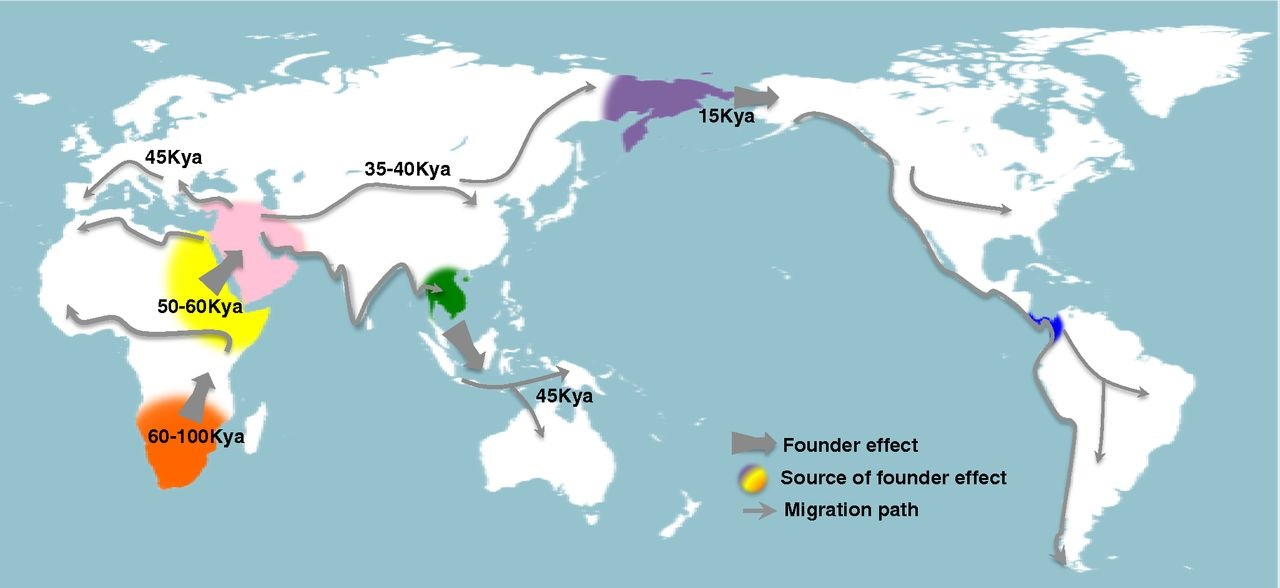
\includegraphics[scale=1.4]{map.jpg}
	}
	\caption[Карта миграции современного человека за последние 100000 лет.]{Карта миграции современного человека за последние 100000 лет. На карте показаны события, которые начались с исходной популяции на юге Африки 60-100 тыс. лет назад и завершились заселением Южной Америки 12-14 тыс. лет назад \autocite{Henn2012}.}\label{fig:map}
\end{figure}

С начала 1900-х годов в антропологии и физиологии возник интерес к вопросу изучения генетической адаптации к высоте более 2500 м, поскольку именно там уровни насыщения кислородом в артериальной крови у большинства людей начинают падать \autocite{Julian2019}. Некоторые из первых исследований проводились в Андах, главным образом в Перу и Боливии. Андские жители произошли от первых поселенцев Америки, которые достигли Южной Америки 15--16 тысяч лет назад, а затем разделились на две ветви. Одна из них обосновалась в прибрежных районах Тихого океана, а другая двинулась вдоль побережья Атлантического океана на восток \autocite{GomezCarballa2018}. 

Первоначально адаптация исследовалась в контексте разделения краткосрочных физиологических реакций, называемых акклиматизацией, и реакций, сохраняющихся независимо от продолжительности пребывания на большой высоте. Модель миграции, представленная в 1960-х годах, использовалась, чтобы различать акклиматизацию, и предполагаемые генетические реакции \autocite{Frisancho1970, Frisancho1995, Frisancho2009}. С появлением технологий исследования однонуклеотидных полиморфизмов выяснилось, что жители Анд и другие высокогорные популяции подверглись естественному отбору в нескольких областях генов, влияющих на чувствительные к кислороду пути \autocite{Moore2017}. Ген EGLN1 был идентифицирован как находящийся под воздействием естественного отбора как у жителей Анд, так и жителей Тибета \autocite{Bigham2009}. SNP в данном гене связывают со снижением концентрации гемоглобина в крови жителей высокогорных регионов \autocite{Beall2010}, а промоторная область EGLN1 полностью располагается внутри острова CpG и регулируется эпигенетически в условиях гипоксии \autocite{Lachance2014}.

Для Тибетского нагорья, типичная высота которого более 4000 м, концентрация кислорода составляет всего $60~\%$ от доступной на уровне моря. Было подтверждено, что уникальный набор физиологических адаптаций к хронической гипоксии, наблюдаемый среди жителей Тибета \autocite{hornbein2001high}, имеют генетическую основу \autocite{Simonson2011, Scheinfeldt2013}. В генах с транскрипционными факторами, индуцируемыми гипоксией (HIF --- Hypoxia-Induced Factors) были обнаружены преобразования изменения концентрации кислорода в изменения экспрессии генов \autocite{Kaelin2008, Lendahl2009, Semenza2012}. Это говорит о том, что у коренных высокогорных популяций отбор для адаптации к хронической гипоксии (в отличие от холода, УФ-излучения или какого-либо другого стресса окружающей среды, испытываемого на большой высоте) является ключевым компонентом их недавней эволюции \autocite{Bigham2014}. В нескольких исследованиях использовалось геномное сканирование для отбора среди тибетцев локусов, мутации в которых являются следствием естественного отбора \autocite{Bigham2009, Simonson2010, Yi2010, Wang2011, Xu2010}. Одним из обнаруженных генов, заслуживающих внимания, является HIF2A, который демонстрирует доказательства положительного направленного отбора (отбор по выгодным мутациям, увеличивающим приспособленность носителей) во всех общегеномных анализах \autocite{Bigham2009, Simonson2010, Yi2010, Wang2011, Xu2010}, а SNP в данном гене в значительной степени связаны с низкой концентрацией гемоглобина у тибетцев \autocite{Yi2010}. Второй ген, показывающий доказательства положительного отбора --- это PHD2 \autocite{Simonson2010, Yi2010, Wang2011, Xu2010}. У тибетцев варианты этого гена связаны с концентрацией гемоглобина, тогда как у жителей Анд такой связи не наблюдалось \autocite{Bigham2009, Simonson2010}. 

Микроэволюция человека под действием низких температур также давно привлекает внимание научного сообщества. В настоящее время этому вопросу посвящён ряд исследований как на уровне всего генома \autocite{Hancock2011adaptations, Cardona2014, Valverde2015}, так и на уровне отдельных регионов или генов \autocite{Ohashi2010, Hancock2010population, Sazzini2014, Quagliarello2017}. Одним из наиболее известных генов с точки зрения его роли в адаптации к холодному климату является TRPM8, расположенный на хромосоме 2. Этот ген отвечает за работу ионного канала в качестве теплового датчика, определяющего температуру в диапазоне 15-30~{\textdegree}C \autocite{Fernandez2011}. Его однонуклеотидные полиморфизмы (SNP) также, считается, могут быть связаны с чувствительностью к холоду \autocite{Kozyreva2011}, реакцией дыхательной системы на охлаждение \autocite{Kozyreva2014}, и антропометрическими параметрами \autocite{Potapova2014}. Также были обнаружены доказательства того, что в гене TRPM8 SNP rs10166942 подвергся климатически обусловленному отбору, что привело к увеличению частоты вариаций его аллелей с юга на север \autocite{Key2018}. Ещё 2 SNP, rs17862920 и rs7577262, связаны с ощущением холодовой боли, причём носители аллеля С (распространены в северных широтах) к ней более восприимчивы. Возможным механизмом дифференциальной выживаемости может быть предотвращение потенциально летальной гипотермии у обладателей аллели С \autocite{Igoshin2019}. 

Таким образом, поиск SNP, связанных с адаптацией человека к сложным климатическим условиям, представляет собой актуальную задачу современной популяционной генетики. Раскрытие механизма их действия на гены может предложить новые терапевтические подходы к лечению различных заболеваний, имеющих схожие с адаптацией к сложным условиям симптомы (например, чувствительность к холоду или гипоксия).

\section{Алгоритмы и методы}\label{sec:ch1/sec2}

\subsection{Регрессионный анализ}\label{subsec:ch1/sec2/subsec1}

Регрессионный анализ представляет собой набор процессов для оценки взаимосвязей между зависимой переменной и одной или несколькими независимыми переменными. Регрессионный анализ в основном используется для двух концептуально различных целей. Во-первых, регрессионный анализ широко используется для прогнозирования, где его использование в значительной степени совпадает с областью машинного обучения. Во-вторых, в некоторых ситуациях регрессионный анализ может использоваться для вывода причинно-следственных связей между независимыми и зависимыми переменными. Наиболее распространённой формой регрессионного анализа является линейная регрессия. В статистике линейная регрессия --- это линейный подход к моделированию взаимосвязи между зависимой переменной и одной или несколькими независимыми переменными. Случай более чем одной независимой переменной называется множественной линейной регрессией \autocite{freedman2009statistical}. 

В линейной регрессии отношения моделируются с использованием функций линейного предсказания, при этом неизвестные параметры модели оцениваются на основе данных \autocite{SEAL1967}. Линейная регрессия была первым типом регрессионного анализа, который получил широкое распространение в практических приложениях \autocite{yan2009linear}. 

Для заданного набора данных $\{y_{i},\,x_{i1},\ldots,x_{ip}\}_{i=1}^{n}$ из $n$ точек модель линейной регрессии предполагает линейную связь между зависимой переменной $y$ и вектором независимых переменных $\textbf{x}$ размера $p$. Если $\varepsilon$ --- случайная ошибка, то модель имеет вид:

\begin{equation}
\label{eq:linreg}
y_{i}=\beta_{0} + \beta_{1} x_{i1} + \cdots + \beta_{p} x_{ip} + \varepsilon_{i} = \mathbf{x}_{i}^{\mathsf{T}}{\boldsymbol{\beta}} + \varepsilon_{i}, \qquad i = 1, \ldots, n.
\end{equation}

В матричной нотации уравнения записываются следующим образом:
\begin{equation}
\label{eq:matrix_linreg}
\mathbf{y}=X{\boldsymbol{\beta}} + {\boldsymbol{\varepsilon}},\,
\end{equation}
где
\begin{equation}
\label{eq:matrix_linreg_vectors}
\mathbf{y} = {\begin{pmatrix} y_{1} \\ y_{2} \\\vdots \\ y_{n} \end {pmatrix}}, \quad X = {\begin{pmatrix} \mathbf{x}_{1}^{\mathsf{T}} \\\mathbf{x}_{2}^{\mathsf{T}} \\\vdots \\\mathbf{x}_{n}^{\mathsf{T}} \end{pmatrix}} = {\begin{pmatrix} 1 & x_{11} & \cdots & x_{1p} \\ 1 & x_{21} & \cdots & x_{2p} \\\vdots & \vdots & \ddots & \vdots \\ 1 & x_{n1} & \cdots & x_{np} \end{pmatrix}},
{\boldsymbol{\beta}} = {\begin{pmatrix} \beta_{0} \\\beta_{1} \\\beta_{2} \\\vdots \\\beta_{p} \end{pmatrix}}, \quad {\boldsymbol{\varepsilon}} = {\begin{pmatrix} \varepsilon_{1} \\\varepsilon_{2} \\\vdots \\\varepsilon_{n} \end{pmatrix}}.
\end{equation}

$\mathbf{y}$ --- вектор наблюдаемых значений $y_{i}\left(i = 1, \ldots, n\right)$ называется зависимой или эндогенной переменной. Решение о том, какая переменная в наборе данных моделируется как зависимая, а какие --- как независимые, принимается в зависимости от природы исходных данных. $X$ можно рассматривать как матрицу векторов-строк $\mathbf{x}_{i}$ или $n$-мерных векторов-столбцов $X_{j}$, которые называются экзогенные переменные, ковариаты, входные переменные или независимые переменные. Константа обычно включается в качестве одного из регрессоров, $\mathbf{x}_{i0} = 1, i = 1, \ldots, n$. Соответствующий элемент $\beta$ называется свободным членом. $\boldsymbol{\beta}$ --- это $(p + 1)$-мерный вектор параметров, где $\beta_{0}$ --- свободный член (если он включён в модель, в противном случае ${\beta}$ $p$-мерный). Его элементы называют коэффициентами регрессии. Элементы этого вектора параметров интерпретируются как частные производные зависимой переменной по различным независимым переменным. ${\boldsymbol{\varepsilon}}$ --- вектор значений $\varepsilon_{i}$, называемых ошибкой или шумом (в отличие от <<сигнала>>, представляемого остальной частью модели). Эта переменная учитывает все другие факторы, которые влияют на зависимую переменную $y$, кроме независимых переменных $x$.
Подгонка линейной модели к заданному набору данных обычно требует оценки коэффициентов регрессии ${\boldsymbol{\beta}}$ так, чтобы минимизировать ошибку ${\boldsymbol{\varepsilon}} = \mathbf{y} - X{\boldsymbol{\beta}}$. Обычно используется сумма квадратов ошибок $||{\boldsymbol{\varepsilon}}||$ как мера качества подгонки.

Стандартные модели линейной регрессии имеют ряд предположений относительно зависимых переменных, независимых переменных и их взаимосвязи:
\begin{itemize}
	\item Слабая экзогенность означает, что независимые переменные $x$ можно рассматривать как фиксированные значения, а не как случайные величины, то есть данные переменные не содержат ошибок измерения. 
	\item Линейность означает, что среднее значение зависимой переменной представляет собой линейную комбинацию коэффициентов регрессии и зависимых переменных. Поскольку зависимые переменные имеют фиксированные значения, линейность является только ограничением для параметров. 
	\item Постоянная дисперсия (гомоскедастичность) означает, что разные значения зависимой переменной имеют одинаковую дисперсию своих ошибок, независимо от значений независимых переменных. 
	\item Независимость от ошибок предполагает, что ошибки зависимых переменных не коррелируют друг с другом. 
	\item Отсутствие идеальной мультиколлинеарности для зависимых переменных --- в стандартном методе наименьших квадратов матрица $X$ должна иметь ранг столбца $p$. 
\end{itemize}

Наиболее распространённым методом построения линейной регрессии является метод наименьших квадратов, в частности OLS (Ordinary Least Squares), который выбирает параметры линейной функции по принципу наименьших квадратов: минимизируя сумму квадратов отклонений между реальными значениями зависимой переменной в данном наборе данных и предсказанными линейной функцией. Геометрически это рассматривается как сумма квадратов расстояний, параллельных оси зависимой переменной, между каждой точкой данных в наборе и соответствующей точкой на линии регрессии --- чем меньше различия, тем лучше модель соответствует данным. Если ошибки имеют нормальное распределение, OLS является оценкой максимального правдоподобия.

Рассмотрим систему:
\begin{equation}
\label{eq:ols}
\sum_{j = 1}^{p} X_{ij} \beta_{j} = y_{i}, \left(i = 1,2, \dots, n\right),
\end{equation}
из $n$ линейных уравнений относительно $p$ неизвестных коэффициентов $\beta_{1}, \beta_{2}, \dots, \beta_{p}$, где $n>p$. В матричной нотации уравнения записываются следующим образом:

\begin{equation}
\label{eq:ols_matrix}
\mathrm{X}{\boldsymbol{\beta}} = \mathbf {y},
\end{equation}
где
\begin{equation}
\label{eq:matrix_ols_vectors}
\mathrm{X} = {\begin{bmatrix}X_{11} & X_{12} & \cdots & X_{1p} \\ X_{21} & X_{22} & \cdots & X_{2p} \\\vdots & \vdots & \ddots & \vdots \\ X_{n1} & X_{n2} & \cdots & X_{np} \end{bmatrix}}, \qquad {\boldsymbol{\beta}} = {\begin{bmatrix} \beta_{1} \\\beta_{2} \\\vdots \\\beta_{p} \end{bmatrix}}, \qquad \mathbf{y} = {\begin{bmatrix}y_{1} \\ y_{2} \\\vdots \\ y_{n} \end{bmatrix}}.
\end{equation}

Такая система обычно не имеет точного решения, поэтому цель состоит в том, чтобы найти коэффициенты $\boldsymbol{\beta}$, которые <<наилучшим образом>> соответствуют уравнениям в смысле решения квадратичной задачи минимизации:
\begin{equation}
\label{eq:ols_minimization}
\hat{\boldsymbol{\beta}} = {\underset{\boldsymbol{\beta}}{\operatorname{arg\,min}}}\,S({\boldsymbol{\beta}}),
\end{equation}
где целевая функция $S$ определяется выражением
\begin{equation}
\label{eq:ols_function}
S({\boldsymbol{\beta}}) = \sum_{i = 1}^{n}{\biggl|} y_{i} - \sum_{j = 1}^{p} X_{ij} \beta_{j} {\biggr|}^{2} = {\bigl\|} \mathbf{y} - \mathrm{X}{\boldsymbol{\beta}}{\bigr\|}^{2}.
\end{equation}
Эта задача минимизации имеет единственное решение при условии, что $p$ столбцов матрицы $X$ линейно независимы, что определяется решением уравнений

\begin{equation}
\label{eq:ols_normal_equations}
(\mathrm{X}^{\mathsf{T}}\mathrm{X}){\hat{\boldsymbol{\beta}}} = \mathrm{X}^{\mathsf{T}}\mathbf{y}.
\end{equation}
$\hat{\boldsymbol{\beta}}$ --- вектор коэффициентов гиперплоскости наименьших квадратов имеет вид
\begin{equation}
\label{eq:ols_betas}
{\hat{\boldsymbol{\beta}}} = \left(\mathrm{X}^{\mathsf{T}} \mathrm{X} \right)^{-1} \mathrm{X}^{\mathsf{T}} \mathbf{y}.
\end{equation}

Предположим, что $b$ является значением <<кандидата>> для вектора параметров $\beta$. Величина $y_i - x_i^T b$, называемая невязкой для $i$-го наблюдения, измеряет расстояние по вертикали между точкой $(x_i, y_i)$ и гиперплоскостью $y = x^T b$, и, таким образом, оценивает степень соответствия между фактическими данными и моделью. Сумма квадратов остатков является мерой соответствия модели:
\begin{equation}
\label{eq:ols_rss}
S(b) = \sum_{i = 1}^{n}(y_{i}-x_{i}^{\mathrm{T}}b)^{2} = (y-Xb)^{\mathrm{T}}(y-Xb),
\end{equation}
где строки $X$, обозначающие значения независимых переменных, связанных с конкретным значением зависимой переменной, равны $X_i = x_i^T$. Функция $S (b)$ является квадратичной по $b$ с положительно определённым гессианом (матрицей вторых производных), и поэтому имеет единственный глобальный минимум при $b ={\hat{\beta}}$:
\begin{equation}
\label{eq:ols_beta}
\hat{\beta} = \operatorname{argmin}_{b \in \mathbb{R}^{p}} S(b) = (X^{\mathrm {T}}X)^{-1} X^{\mathrm{T}}y.
\end{equation}

Предсказанные значения линейной регрессии будут иметь вид:
\begin{equation}
\label{eq:ols_y}
\hat{y} = X{\hat{\beta}}.
\end{equation}
Обычно модель линейной регрессии оценивают путём сравнения того, насколько первоначальная дисперсия в выборке может быть уменьшена при построении регрессии с помощью коэффициента детерминации $R^2$. Если $\bar{y}$ --- это среднее значение наблюдаемых данных:
\begin{equation}
\label{eq:ols_mean}
\bar{y} = {\frac{1}{n}} \sum_{i = 1}^{n} y_{i},
\end{equation}
тогда вариабельность набора данных может быть измерена с помощью двух формул суммы квадратов:
\begin{itemize}
	\item Общая сумма квадратов: $SS_{\text{tot}} = \sum_{i} (y_{i} - {\bar{y}})^{2}$
	\item Сумма квадратов остатков: $SS_{\text{res}} = \sum_{i} (y_{i}-f_{i})^{2} = \sum_{i} e_{i}^{2}$
\end{itemize}
Наиболее общее определение коэффициента детерминации:
\begin{equation}
\label{eq:ols_r2}
R^{2} \equiv 1- {SS_{\text{res}} \over SS_{\text{tot}}}
\end{equation}
В лучшем случае смоделированные значения точно соответствуют наблюдаемым, что приводит к $SS_{\text{res}} = 0$ и $R^{2} = 1$. 

\subsection{Обучение с учителем}\label{subsec:ch1/sec2/subsec2}

Обучение с учителем --- это задача машинного обучения, состоящая в построении функции, которая сопоставляет входные данные с выходными на основе примеров пар <<стимул-реакция>> \autocite{russell2010artificial}. При обучении с учителем каждый пример представляет собой пару, состоящую из входного объекта (обычно вектора) и желаемого выходного значения. Алгоритм обучения с учителем анализирует входные данные и создаёт предполагаемую функцию, которую можно использовать для отображения новых примеров. Оптимальный сценарий позволит алгоритму правильно определять метки классов для неизвестных входов. 

Основные этапы решения задачи обучения с учителем:
\begin{enumerate}
	\item Определение типа обучающих примеров --- необходимо принять решение, какие данные будут использоваться в качестве обучающей выборки. 
	\item Сбор обучающей выборки --- входных объектов и соответствующих выходных данных, полученных на основе измерений.
	\item Определение представления входных данных. Обычно входной объект преобразуется в вектор признаков, который содержит ряд функций, описывающих объект. Количество признаков не должно быть слишком большим, но должно содержать достаточно информации, чтобы точно предсказать результат.
	\item Определение структуры изучаемой функции и соответствующего алгоритма обучения. 
	\item Запуск алгоритма обучения на тренировочной выборке, при необходимости определение параметров управления. 
	\item Оценка точности построенной функции. После настройки параметров и обучения производительность результирующей функции должна быть измерена на отдельном тестовом наборе данных.
\end{enumerate}

Пусть дан набор из $N$ тренировочных примеров в виде $\{(x_1, y_1), ..., (x_N,\; y_N)\}$ таких, что $x_{i}$ --- вектор признаков $i$-го примера, а $y_{i}$ --- его метка (например, класс). Алгоритм обучения ищет функцию $g: X \to Y$, где $X$ --- пространство входных данных, а $Y$ --- выходных данных. Функция $g$ является элементом некоторого пространства допустимых функций $G$, обычно называемого пространством гипотез. Иногда $g$ представляют с помощью функции оценки $f: X \times Y \to \mathbb{R}$ таким образом, что $g$ определяется как возвращаемое значение $y$, которое даёт лучший результат: $g(x) = {\underset{y} {\arg\max}}\; f(x, y)$. $F$ обозначает пространство функций оценки. Несмотря на то, что $G$ и $F$ могут быть любыми пространствами функций, многие алгоритмы обучения являются вероятностными моделями, где $g$ принимает форму модели условной вероятности $g(x) = P(y|x)$ или $f$ принимает форму совместного распределения $f(x, y) = P(x, y)$. 

Существует два основных подхода к выбору $f$ или $g$: минимизация эмпирического риска и минимизация структурного риска \autocite{vapnik2013nature}. Минимизация эмпирического риска ищет функцию, которая лучше всего соответствует обучающим данным. Минимизация структурного риска включает функцию штрафа. В обоих случаях предполагается, что обучающий набор состоит из выборки независимых и одинаково распределённых пар $(x_i, \; y_i)$. Чтобы измерить, насколько хорошо функция соответствует обучающим данным, вводится функция потерь $L: Y \times Y \to \mathbb {R}^{\geq 0}$. Для примера $(x_i, \; y_i)$ значение функции потерь для предсказанного значения $\hat{y}$ представляется как $L(y_i,\hat{y})$. Риск $R (g)$ функции $g$ определяется следующим образом:
\begin{equation}
\label{eq:sup_learn_loss}	
R_{emp} (g) = \frac{1}{N} \sum_i L(y_i, g(x_i)).
\end{equation}

При минимизации эмпирического риска алгоритм обучения с учителем ищет функцию $g$, которая минимизирует $R (g)$. Следовательно, алгоритм обучения с учителем может быть построен путём применения некоторого метода оптимизации для нахождения $g$. Когда $g$ --- условное распределение вероятностей $P (y | x)$, а функция потерь $L(y, \hat{y}) = -\log P(y | x)$, то минимизация эмпирического риска эквивалентна оценке максимального правдоподобия. Когда $G$ содержит много функций-кандидатов или обучающая выборка недостаточно велика, минимизация эмпирического риска приводит к высокой дисперсии и плохому обобщению. Алгоритм обучения способен запоминать обучающие примеры без хороших обобщений --- это называется переобучением.

Минимизация структурных рисков направлена на предотвращение переобучения за счёт добавления штрафа регуляризации. Например, рассмотрим случай, когда функция $g$ является линейной функцией вида
\begin{equation}
\label{eq:sup_learn_risk}
g(x) = \sum_{j = 1}^d \beta_j x_j.
\end{equation}
Часто используемым штрафом регуляризации является $\sum_j \beta_j^2$, который представляет собой квадрат евклидовой нормы весов, также известный как норма $L_{2}$. Другие нормы включают норму $L_{1}$, $\sum_j |\beta_j|$ и $L_{0}$, которая представляет собой количество ненулевых $\beta_{j}$. Штраф обозначается $C (g)$. Задача оптимизации обучения с учителем состоит в том, чтобы найти функцию $g$, которая минимизирует
\begin{equation}
\label{eq:sup_learn_opt}
J(g) = R_{emp}(g) + \lambda C(g).
\end{equation}
Параметр $\lambda$ управляет соотношением смещения и дисперсии. Когда $\lambda = 0$, имеем минимизацию эмпирического риска с низким смещением и высокой дисперсией. Когда $\lambda$ велико, алгоритм обучения будет иметь высокое смещение и низкую дисперсию. 

Наиболее распространёнными методами обучения с учителем являются искусственные нейронные сети, метод обратного распространения ошибки, байесовкие классификаторы, методы $k$-ближайших соседей, ансамбли классификаторов, машины опорных векторов и многие другие. Своё применение данные методы находят в таких областях науки и техники, как биоинформатика, хемоинформатика, распознавание образов, компьютерное зрение, извлечение информации. 

\subsection{Метод построения случайного леса}\label{subsec:ch1/sec2/subsec3}

Случайные леса (Random Forest) --- это метод обучения ансамбля для решения задач классификации и регрессии, работающий путём построения множества деревьев решений во время обучения \autocite{TinKamHo1998}. Случайный лес корректирует деревья решений пир попытке переобучаться на обучающей выборке \autocite{hastie2001elements}. Первый алгоритм построения случайных лесов был предложен Тином Кам Хо с использованием метода случайных подпространств \autocite{TinKamHo1998}, расширение алгоритма было разработано Лео Брейманом \autocite{Breiman2001} на основе идеи бутстрэп-агрегирования для построения набора деревьев решений с контролируемой дисперсией. Общий метод предполагает, что леса из деревьев решений, расщепляющиеся наклонными гиперплоскостями, могут наращивать точность по мере роста, не страдая от переобучения, до тех пор, пока леса случайным образом ограничены, чтобы быть чувствительными только к выбранным признакам. Устойчивость метода леса к переобучению объясняется теорией стохастической дискриминации Клейнберга \autocite{Kleinberg1990, Kleinberg2000}. 

Деревья решений --- популярный метод решения различных задач машинного обучения. Их структура подобна блок-схеме, в которой каждый внутренний узел представляет некоторый <<тест>>, каждая ветвь представляет результат теста, а каждый листовой узел представляет собой метку класса. Пути от корня к листу представляют собой правила классификации. Дерево решений состоит из трёх типов узлов \autocite{Kamiski2017}: узлы решения, вероятностные узлы, замыкающие узлы. Обучение дерева решений --- один из подходов к моделированию, используемых в статистике, интеллектуальном анализе данных и машинном обучении. Модели деревьев, в которых целевая переменная может принимать дискретный набор значений, называются деревьями классификации; в этих древовидных структурах листья представляют метки классов. Деревья решений, в которых целевая переменная может принимать непрерывные значения, называются деревьями регрессии. Слишком глубокие деревья решений склонны к переобучению. Случайные леса --- это способ усреднения нескольких глубоких деревьев решений, обученных на разных частях одной и той же обучающей выборки, с целью уменьшения дисперсии \autocite{hastie2001elements}. Леса подобны объединению усилий отдельных деревьев решений.

Алгоритм обучения для случайных лесов применяет общую технику бутстрэп-агрегирования. Для заданной обучающей выборки $X = x_1, ..., x_n$ с ответами $Y = y_1, ..., y_n$, бутстрэп-агрегирование многократно ($B$ раз) заменяет обучающую выборку случайной и применяет деревья к этим выборкам. Для $b = 1, ..., B$ алгоритм сначала выбирает с заменой $n$ обучающих примеров из $X, Y$ ($X_b, Y_b$), затем обучает дерево классификации или регрессии $f_b$ на $X_b, Y_b$. После обучения прогнозы для непросмотренных выборок $x'$ могут быть сделаны путём усреднения прогнозов всех отдельных деревьев:
\begin{equation}
\label{eq:rf_bagging}
\hat{f} = {\frac{1}{B}} \sum_{b = 1}^{B} f_{b} (x')
\end{equation}
в случае регрессии или путём получения большинства голосов в случае деревьев классификации.

Эта процедура приводит к лучшей производительности модели, потому что она уменьшает её дисперсию без увеличения смещения. Это означает, что, несмотря на чувствительность прогнозов одного дерева к шуму, среднее значение для многих деревьев таковым не будет, если деревья не коррелированы. Простое обучение множества деревьев на одном обучающем наборе даст сильно коррелированные деревья (или одно и то же дерево много раз, если алгоритм обучения детерминирован), а бутстрэп-аггрегирование --- это способ декоррелировать деревья, показывая им разные обучающие наборы. Кроме того, оценка неопределённости прогноза может быть сделана на основе стандартного отклонения прогнозов по всем отдельным деревьям:
\begin{equation}
\label{eq:rf_error}
\sigma = {\sqrt{\frac{\sum_{b = 1}^{B} (f_{b} (x') - {\hat{f}})^{2}} {B-1}}}.
\end{equation}
Количество деревьев $B$ является свободным параметром. Обычно используется от нескольких сотен до нескольких тысяч деревьев, в зависимости от размера и характера обучающей выборки. Случайные леса используют модифицированный алгоритм обучения деревьев, который выбирает при каждом разбиении в процессе обучения случайное подмножество признаков. Если один или несколько признаков являются очень сильными предикторами для переменной ответа, эти признаки будут выбраны во многих деревьях, делая их коррелированными. Как правило, для задачи классификации с $p$ признаками в каждом разбиении используются $\sqrt{p}$ признаков, для задач регрессии --- $p / 3$. На практике наилучшие значения для этих параметров будут зависеть от задачи, и их следует подбирать отдельно.

Случайные леса можно использовать для ранжирования важности переменных в задаче регрессии или классификации. Первый шаг в измерении важности переменной в наборе данных $\mathcal{D}_{n} = \{(X_{i}, Y_{i}) \}_{i = 1}^{n}$ состоит в применении случайного леса к данным. Для каждой точки запоминается out-of-bag ошибка --- средняя ошибка предсказания для каждой обучающей выборки $x_i$ с использованием только тех деревьев, у которых не было $x_i$ в их начальной выборке, затем эта ошибка усредняется по лесу. Чтобы измерить важность $j$-го признака после обучения, значения $j$-го признака переставляются среди обучающей выборки, и снова вычисляется out-of-bag ошибка. Оценка важности $j$-го признака вычисляется путём усреднения разницы out-of-bag ошибок до и после перестановки по всем деревьям. Оценка нормализуется на стандартное отклонение этих различий. Признаки, имеющие более высокие значения этой оценки, ранжируются как более важные \autocite{Zhu2015tree}. Однако, этот метод определения важности признаков имеет ряд недостатков. Для данных, включающих категориальные переменные с разным количеством уровней, случайные леса будут смещены в пользу признаков с большим количеством уровней. Для решения этой проблемы можно использовать такие методы, как частичные перестановки \autocite{Altmann2010} и несмещённые деревья \autocite{Strobl2007}. Если данные содержат группы коррелированных характеристик, имеющих одинаковую значимость для ответа, то группы меньшего размера будут предпочтительнее \autocite{Toloi2011}.

\subsection{Метаанализ}\label{subsec:ch1/sec2/subsec4}

Метаанализ --- это статистический анализ, объединяющий результаты нескольких научных исследований. Метаанализ может быть выполнен, когда есть несколько исследований, посвящённых одному и тому же вопросу, причём ожидается, что измерения каждого отдельного исследования имеют некоторую степень ошибки. Цель состоит в том, чтобы использовать статистические подходы для получения объединённой оценки. Существующие методы метаанализа позволяют получить средневзвешенное значение по результатам отдельных исследований. Метаанализ также может сопоставить результаты различных исследований и выявить закономерности среди результатов, источники разногласий между ними или другие интересные взаимосвязи, которые могут выявиться в контексте нескольких исследований.

Ключевым преимуществом этого подхода является агрегирование информации, приводящее к более высокой статистической мощности и более надёжной оценке, чем при использовании любого отдельного исследования. Однако, при выполнении метаанализа выбор рассматриваемых исследований может повлиять на итоговый результат \autocite{WALKER2008}. Метаанализ часто является важным компонентом  систематического обзора. Например, он может быть проведён по нескольким клиническим испытаниям медицинского препарата, для лучшего понимания, насколько хорошо работает лечение. 

Общие шаги заключаются в следующем:
\begin{enumerate}
	\item Формулировка основного вопроса исследования, изучение литературы.
	\item Выбор исследований: на основе критериев качества (требование рандомизации и слепого контроля в клиническом исследовании), по определённой тематике.
	\item Определение зависимых переменных: различия между исследованиями (в случае дискретных данных), средние значения (в случае непрерывных данных).
	\item Выбор модели метаанализа.
	\item Изучение источников неоднородности между исследованиями.
\end{enumerate}

Наиболее распространены два основных типа моделей метаанализа: с фиксированными эффектами и со случайными эффектами. Модель с фиксированным эффектом обеспечивает средневзвешенное значение наблюдаемых. В качестве веса исследования обычно используется величина, обратная дисперсии наблюдаемых, поэтому более крупные исследования, как правило, вносят больший вклад в средневзвешенное значение. Следовательно, когда в исследованиях в рамках метаанализа есть очень большое исследование, результаты небольших исследований практически игнорируются \autocite{Helfenstein2002}. Модель c фиксированными эффектами предполагает, что все включённые исследования рассматривают одну и ту же популяцию, используют одни и те же переменные и выходные данные. Это предположение обычно нереалистично, поскольку исследования зачастую имеют несколько источников неоднородности, например эффекты лечения могут различаться в зависимости от региона, уровней дозировки, условий исследования и т.д. В большинстве случаев для объединения гетерогенных исследований используют модель метаанализа со случайными эффектами --- средневзвешенное значение величины эффекта группы исследований. Поскольку в данном случае вес не зависит от размера выборки, перевеса в пользу более крупного исследования не происходит. 

Современный статистический метаанализ может проверить, являются ли результаты исследований более вариабельными, чем ожидается, из-за выборок разного размера. Другие виды использования метааналитических методов включают разработку и проверку моделей клинического прогнозирования, где метаанализ может использоваться для объединения данных отдельных участников из разных исследовательских центров и для оценки обобщения модели \autocite{Debray2015}. 

В генетике метаанализ полногеномного поиска ассоциаций, в отличие от анализа объединённых данных на индивидуальном уровне, позволяет избежать интеграции генотипических и фенотипических данных из разных исследований. Было показано, что метаанализ столь же эффективен (с точки зрения статистической мощности), как и объединение данных на индивидуальном уровне из разных исследований \autocite{Lin2009}. Одним из основных подходов к доказательству существования ассоциаций между отдельными исследованиями является преобразование направления эффекта и P-значения, наблюдаемых в каждом исследовании, в Z-значение. Большие отрицательные Z-значения указывают на низкий риск заболевания или уровень количественного признака, тогда как большие положительные Z-значения указывают на высокий риск заболевания или уровень количественных признаков \autocite{Willer2010}. Z-значения для каждого аллеля объединяются по выборкам во взвешенную сумму с весами, пропорциональными квадратному корню из размера выборки для каждого исследования:
\begin{equation}
\label{eq:metal_z}
Z=\frac{\sum_{i}Z_i w_i}{\sqrt{\sum_{i}w_i^2}},
\end{equation}
где $w_i = \sqrt{N_i}$, $Z_i = \Phi^{-1}\left(P_i/2\right) * \text{sign}(\delta_i)$, $N_i$ --- размер выборки, $P_i$ --- P-значение, $\delta_i$ --- направление для исследования $i$. Итоговое P-значение вычисляется в соответствии с формулой:
\begin{equation}
\label{eq:metal_p}
P = 2\Phi \left(|-Z|\right).
\end{equation}

В дальнейшем используется полученное p-значение, которое характеризует суммарный эффект всех рассматриваемых исследований. 

\section{Задачи, решаемые в диссертационном исследовании}\label{sec:ch1/sec3}

Из проведённого обзора следует, что существующие в настоящее время статистические методы анализируют генетические данные с точки зрения ассоциации либо только с непрерывными переменными (возраст, рост, вес), либо только с категориальными (пол, подверженность вредным привычкам), не рассматривая совместное влияние непрерывных и категориальных переменных. Проведение полногеномного анализа требует разработки метода сокращения размерности, а также оптимизации существующих алгоритмов.

На основании выполненного обзора определим цель работы: разработка и программная реализация методов статистического анализа экспериментальных генетических и эпигенетических данных для оценки физиологического состояния человека.

Основные задачи диссертационного исследования:
\begin{enumerate}
	\item Разработка и программная реализация метода поиска связанных с возрастом специфичных для пола биомаркеров на основе анализа экспериментальных эпигенетических данных.
	\item Разработка и программная реализация метода поиска биомаркеров с возрастной вариабельностью, связанной с полом, на основе анализа экспериментальных эпигенетических данных. 
	\item Разработка и программная реализация метода анализа экспериментальных митохондриально-ядерных генетических данных для оценки региональных различий адаптации к климатическим условиям. 
\end{enumerate}

\section*{Выводы по главе 1} \label{sec:ch1/conclusion}                       
\addcontentsline{toc}{section}{Выводы по главе 1}    

В первой главе был проведён обзор предметной области и результатов существующих исследований, посвящённых статистическому анализу генетических и эпигенетических данных. Также в первой главе приведена терминология и результаты современной математической статистики, теории машинного обучения и информатики, которые требуются для описания представляемых в диссертационной работе методов и алгоритмов.

В главе приведены определение дезоксирибонуклеиновой кислоты (ДНК), даны описание её структуры, перечислены виды и основные функции. Дано определение однонуклеотидного полиморфизма, описано влияние точечных мутаций на адаптацию человеческого организма к сложным климатическим условиям (экстремально низкие температуры, высокогорный климат с низкой концентрацией кислорода в воздухе). Рассмотрен один из наиболее широко изучаемых в настоящее время эпигенетических факторов --- метилирование ДНК, показаны его свойства и воздействия на физиологическое состояние человека. Приведены работы, в которых исследуется зависимость уровня метилирования отдельных участков ДНК от возраста, пола и других ковариатов. После этого приведены основные математические методы анализа, применяемые к генетическим и эпигенетическим данным: построение регрессионной модели, задача обучения с учителем и, в частности, построение случайного леса деревьев решений, а также метаанализ. Регрессионные модели успешно применяются к задачам поиска биомаркеров с определённым законом зависимости от выбранных биологических параметров, а при объединении данных из разнородных исследований применяется метаанализ. Поскольку полногеномный анализ подразумевает работу с большими объёмами данных, для анализа применяются классические методы машинного обучения.

Наконец, определена цель диссертационного исследования как разработка и программная реализация методов статистического анализа экспериментальных генетических и эпигенетических данных для оценки физиологического состояния человека, а также поставлены конкретные задачи, позволяющие достичь сформулированной цели.


\FloatBarrier
